\documentclass[10pt,a4paper]{article}
\usepackage[margin=20mm,headheight=14pt,footskip=10mm]{geometry}
\usepackage[T1]{fontenc}
\usepackage{lmodern,microtype,amsmath,amssymb,booktabs,tabularx,array}
\usepackage{graphicx,xcolor,tikz,caption,enumitem,fancyhdr,hyperref}
\usetikzlibrary{arrows.meta,positioning,calc,fit}
\definecolor{ink}{HTML}{193348}
\definecolor{accent}{HTML}{006B73}
\definecolor{muted}{HTML}{526574}
\definecolor{wash}{HTML}{EAF2F4}
\hypersetup{colorlinks=true,linkcolor=accent,citecolor=accent,urlcolor=accent,
 pdftitle={From cue activity to defensible condition-level decoding},
 pdfauthor={Hongyi's neuroscience workspace}}
\pagestyle{fancy}\fancyhf{}
\fancyhead[L]{\small\color{muted}Hippocampal cue decoding: research synthesis}
\fancyhead[R]{\small\color{muted}15 November 2026}
\fancyfoot[C]{\small\thepage}
\renewcommand{\headrulewidth}{0.3pt}
\setlength{\parindent}{0pt}\setlength{\parskip}{5pt}
\setlength{\tabcolsep}{5pt}
\renewcommand{\arraystretch}{1.14}
\captionsetup{font=small,labelfont=bf,labelsep=period,skip=5pt}
\setlist{nosep,leftmargin=16pt}
\newcolumntype{L}[1]{>{\raggedright\arraybackslash}p{#1}}
\newcolumntype{Y}{>{\raggedright\arraybackslash}X}
\newcommand{\BA}{\operatorname{BA}}
\newcommand{\pp}{\,\mathrm{pp}}
\newcommand{\repo}[2]{\href{https://github.com/Hong-yiii/neuro_science/blob/a0ca80180e2bb52b90e499357d3d6965b26806da/#1}{#2}}
\newcommand{\key}[1]{\vspace{3pt}\noindent\colorbox{wash}{\parbox{\dimexpr\linewidth-2\fboxsep\relax}{\small #1}}\vspace{3pt}}
\newcommand{\figurefile}[2][]{\includegraphics[#1]{figures/#2}}

\begin{document}
\thispagestyle{empty}
{\small\color{accent}\textbf{RESEARCH SYNTHESIS}\hfill Evidence through 15 November 2026}\par
\vspace{5mm}
{\LARGE\bfseries\color{ink}From cue activity to defensible\par condition-level decoding}\par
\vspace{3mm}
{\large Source support, population construction and the evolution of a hippocampal research series}\par
\vspace{2mm}
{\small Hongyi's neuroscience workspace \quad\textbullet\quad Exploratory evidence synthesis}

\begin{abstract}
\noindent This repository investigates what hippocampal cue-period recordings can reveal about a navigation task and what learned representations permit us to claim. Its progression is chiefly methodological: from aligning recordings and defining path targets, through failures of source transfer and comparisons of simple and learned features, to explicit experiments on the construction of cross-session pseudopopulations. The most recent study holds nine ordered start--goal classes fixed, compares two, three and five distinct training sources at 17 recorded columns, and then expands nested rosters to 49 and 83 columns at three sources per session--class pool. Raw and principal-component features with support-vector readouts retain endpoint association when each selected training source is used once. Additional sources and wider rosters affect pipelines differently: PCA/SVM mean pair balanced accuracy rises from 33.33\% to 68.06\% to 72.22\%, although the final step improves only one of three computational repeats. Neither repeated assembly nor CEBRA has a universal advantage. A complete notebook reproduction matches the accepted numerical results, establishing computational repeatability on the same recordings, not new biological replication. Known-label construction, historically exposed development data, source dependence and incomplete acquisition metadata bound the inference. The evidence supports conditional endpoint decoding and a clearer account of its construction; it does not establish ordered-path recovery, simultaneous population dynamics or a generally reusable neural state.
\end{abstract}

\section{The question changed because the evaluation object mattered}
The original ambition was to ask whether activity during the cue predicts the subsequent \emph{path} beyond its start and goal, and whether that information has reproducible low-dimensional organization. A path is an ordered movement through the maze. An ordered endpoint pair is a much coarser label: several different paths can share it. A binary indicator of visiting one interior path component is different again. Much of the series was needed to separate these targets and to establish which measurement and evaluation objects the recordings could support \cite{history,contract}.

The central object is a \emph{pseudopopulation}: a vector assembled from recordings made in different sessions, choosing contributions that share a known task condition. Such an object can test condition-level response differences. It is not a population measured during one natural trial. The label is used to build the vector before a decoder predicts that label; consequently, a successful decoder evaluates a conditional assay, not an operational system that receives an unknown trial and discovers its condition. Source separation is necessary for this assay, but does not remove that distinction.

This paper integrates the completed series rather than reporting a new experiment. Older work supplies the reasons for the current design; November's support, reuse and width studies supply the main quantitative evidence. The source cutoff is the completed experiment in PR~31, revision \texttt{a0ca801} \cite{latest}. All numerical displays are extracted or replotted from existing published aggregate outputs. No fitting, raw-data reconstruction, model replay, new literature search or additional biological analysis was performed for this synthesis.

\key{\textbf{Reading rule.} Recorded spikes are measurements. Counts, constructed populations and embeddings are derived objects. Decoding is an association under a declared evaluation procedure. Each step needs its own justification.}

\clearpage
\section{From recorded events to a conditional population assay}
The archive contains sorted-unit spike timestamps, Ripple neural-clock task events, Eyelink events and Unity task records. The compact source release contains 195 selected units and 58 sessions; this is an archive inventory, not the size of every analyzed population. A sorted unit is a curated extracellular spike source, not a verified anatomical cell identity. Selection was place-oriented, so this is not an unbiased sample of hippocampal neurons. Species, subject count, session-to-subject mapping, recording subfields and definitive simultaneity groups remain insufficiently documented for population-level biological generalization \cite{data}.

The task has six start/goal categories, normally yielding 30 distinct ordered pairs when start and goal differ. Marker semantics and the previous-goal/current-start rule provide provisional endpoint labels; this is not a direct measurement of intention. A \emph{source trial} here is one recorded current trial within a session. The successful-after-successful subset retains a trial only when both it and its immediate predecessor succeeded; the predecessor's goal supplies the operational start label. Thus different current-trial IDs can still share contributing information. Cue identity, visual input, gaze and preceding-trial state may covary with endpoints; these assays do not separate all such explanations \cite{contract,data}.

\begin{figure}[h!]
\centering
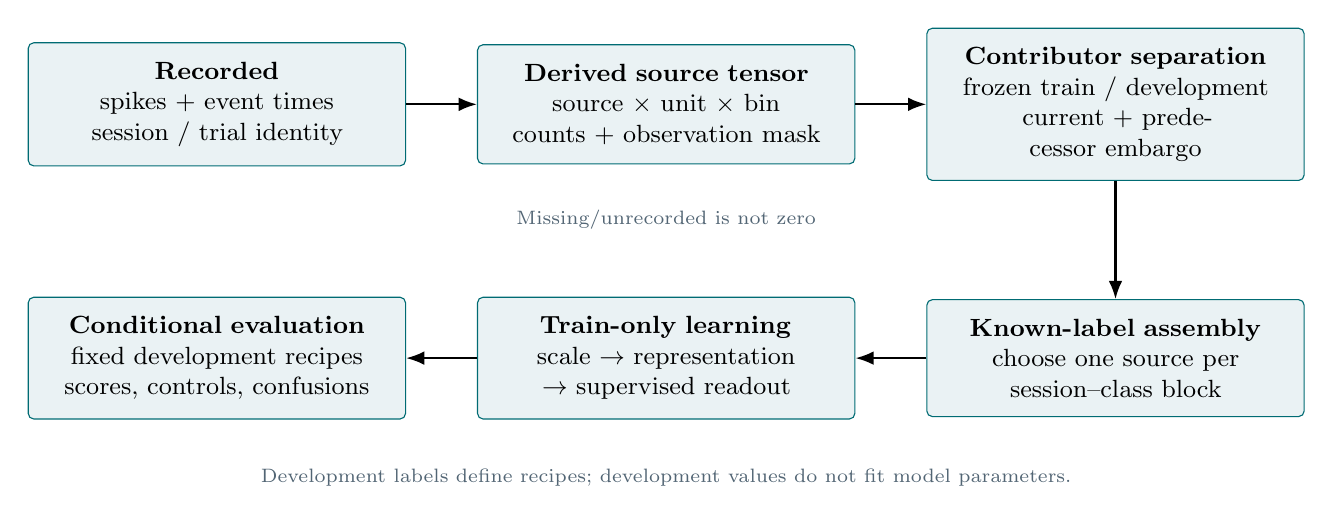
\begin{tikzpicture}[font=\small,>=Latex,
 box/.style={draw=accent,rounded corners=2pt,fill=wash,align=center,inner sep=7pt,text width=43mm},
 lab/.style={font=\scriptsize,text=muted,align=center}]
\node[box] (raw) {\textbf{Recorded}\par spikes + event times\par session / trial identity};
\node[box,right=9mm of raw] (source) {\textbf{Derived source tensor}\par source $\times$ unit $\times$ bin\par counts + observation mask};
\node[box,right=9mm of source] (split) {\textbf{Contributor separation}\par frozen train / development\par current + predecessor embargo};
\node[box,below=15mm of split] (assembly) {\textbf{Known-label assembly}\par choose one source per\par session--class block};
\node[box,left=9mm of assembly] (model) {\textbf{Train-only learning}\par scale $\to$ representation\par $\to$ supervised readout};
\node[box,left=9mm of model] (score) {\textbf{Conditional evaluation}\par fixed development recipes\par scores, controls, confusions};
\draw[->,thick] (raw)--(source);
\draw[->,thick] (source)--(split);
\draw[->,thick] (split)--(assembly);
\draw[->,thick] (assembly)--(model);
\draw[->,thick] (model)--(score);
\node[lab] at ($(source.south)+(0,-7mm)$) {Missing/unrecorded is not zero};
\node[lab,below=5mm of model] {Development labels define recipes; development values do not fit model parameters.};
\end{tikzpicture}
\caption{Measurement-to-assay schematic for the latest study, not a data plot. The global contributor embargo is applied before panel selection. Within a selected session block, all retained columns and all ten cue bins follow the same source trial. Grouping preserves recorded source identity; it does not independently verify simultaneity. Sources: the analysis contract and frozen latest protocol \cite{contract,latest}.}
\label{fig:pipeline}
\end{figure}

For source $i$, unit $u$ and cue bin $b$, the observed count is
\begin{equation}
 x_{iub}=\sum_{t\in\mathcal T_u}\mathbf 1\{t_i+0.1b\leq t<t_i+0.1(b+1)\},\qquad b=0,\ldots,9,
\label{eq:count}
\end{equation}
where $\mathcal T_u$ contains spike times in seconds and $t_i$ is cue onset in the neural clock. An observation mask distinguishes unavailable source--unit entries from measured zero spikes. The one-second cue becomes ten half-open 100-ms bins; matching array dimensions alone is not evidence of clock alignment.

For class $c$, a recipe selects source $i(r,s,c)$ for each session block $s$ of constructed row $r$. Its columns are concatenated as
\begin{equation}
 \widetilde X_{r,:,b}=\bigoplus_{s=1}^{S}X_{i(r,s,c),U_s,b},
\label{eq:assembly}
\end{equation}
with $U_s$ the recorded columns retained from session $s$. This preserves within-source structure while creating cross-session combinations. It cannot reconstruct missing cross-session noise covariance or the trajectory of one simultaneous neural population. Sources, sessions, bins, constructed rows and computational seeds are therefore different counting units.

\clearpage
\section{How the series reached the current experiment}
The research trajectory is a succession of more precise questions, not a monotonic sequence of better scores. Table~\ref{tab:history} records the main transitions. Each transition changes the interpretation of the evaluation; several also change its population, target or feature construction.

\begin{table}[h!]
\caption{Evidence progression. Earlier work is context, not additional replication of the latest study. Dates denote the research series, not acquisition dates.}
\label{tab:history}\small
\begin{tabularx}{\linewidth}{L{23mm}Y Y}
\toprule
Stage & Completed contribution & Consequence for interpretation \\
\midrule
July--August & Lab-code onboarding; navigation export, marker and source-identity audits; review of earlier student analyses. & A spatial-bin export and a cue-period population are different inputs. The prior 233-cell pseudopopulation is distinct from the 195-unit archive. \\
September & Source-declared graph-component assays, source-transfer tests and preprocessing/readout controls. & Recombining known sources can look much stronger than transfer to held-out sources. Attractive embeddings do not establish path information. \\
Late September--October & Matched raw/PCA/CEBRA and decoder comparisons; cue-only versus cue/navigation training; cue-window and endpoint readouts. & Endpoint association is clearer than robust path evidence; representation, decoder and evaluation window must be distinguished. \\
October 23--27 & Independent source reconstruction, a 27-unit/10-session panel, reusable APIs and teaching notebooks. & Stronger contributor accounting and support restrictions change the cohort; historical scores are not portable accuracy guarantees. \\
November 10--11 & Explicit source-use controls, then three class sets $\times$ three rosters and four readouts; saved-result error analysis. & Learning can survive once-only assembly. Class deletion changes the task; reuse is entangled with available source coverage. \\
November 14--15 & Fixed nine-class source-budget and nested-width study; full executed notebook reproduction. & Sampling effects can be compared within one task, while repeated rows, added sessions and computational replication remain distinct. \\
\bottomrule
\end{tabularx}
\end{table}

The early source-transfer work exposed the danger of treating novel combinations as novel measurements. In the 29-unit/seven-session, fixed-$4\to3$ binary path-component assay, CEBRA-Time gave 99.25\% mean balanced accuracy on new mixtures of training sources but 24.92\% on the exact development-source combinations. Those evaluations use different source pools and construction measures; their gap does not identify one cause \cite{path}. Later matched raw/PCA preprocessing comparisons found limited signal without broad robustness across diagnostics. Neither a negative configured CEBRA result nor a favorable linear baseline proves the absence of path coding. Ordered-route prediction was not completed, and the artificial-agent comparison was removed from active scope \cite{history,contract}.

In the October endpoint study, a 195-unit/58-session construction gave mean whole-cue pair balanced accuracies of 70.28\% for raw features, 83.61\% for PCA, 63.75\% for cue-only CEBRA-Time and 75.56\% for joint cue/navigation CEBRA, with the same logistic readout. These are three-repeat summaries on exposed development pseudopopulations. Joint training helped that cue-only comparison, but changed phase content and cue exposure; it did not establish general joint-training superiority or a shared biological geometry \cite{endpoint}. Window-specific classifiers were also fitted, whereas a matched frozen CEBRA train-time $\times$ test-time transfer analysis remained unexecuted.

The October 23 panel instead used 27 units, 10 sessions and 1,415/551 available training/development sources after the stricter global contributor embargo and support selection. Its two-repeat full-pool pair means were 16.88\% raw, 13.33\% PCA and 17.08\% CEBRA with logistic readouts \cite{fresh}. This is not a longitudinal performance collapse: cohort, source protection and pipeline details differ. It made source support and construction policy central questions rather than nuisances to hide behind a single score.

\clearpage
\section{The recent design separates budgets, rows and width}
November 10 first compared smaller endpoint panels, balanced allocation, fewer columns and once-only use. On its 80-unit/20-session nine-class panel, once-only Raw/PCA/Time logistic pair means were 47.22/54.17/31.94\%, respectively, each with all three observed repeats above the five corresponding label-world controls. Repeating those same sources five times changed PCA by $-9.72\pp$ and Time by $+7.87\pp$: even then, repetition was pipeline-dependent \cite{support}.

November 11 replaced that design with \emph{three class requirements by three session rosters}, not a nine-class endpoint rectangle. Its nine populations spanned 8--138 columns and 15/20/30 classes. All retained a two-source training bottleneck. Once-only assembly, repeated use of the same sources, and fuller source coverage supported within-task comparisons. Wider rosters did not uniformly help: full-pool PCA/SVM means fell 19.03$\to$15.42$\to$10.28\% for the 30-class task, but rose 50.56$\to$73.06$\to$81.11\% for the 15-class task. Changing class sets also changed the task and eligible population \cite{grid}.

The latest study therefore fixes nine ordered pairs:
\[
\mathcal C=\{1\!\to\!2,1\!\to\!4,2\!\to\!5,2\!\to\!6,3\!\to\!1,4\!\to\!6,5\!\to\!3,5\!\to\!4,6\!\to\!2\}.
\]
This is a sparse endpoint panel, not a Cartesian $3\times3$ grid and not nine measured paths. A \emph{pool} contains eligible sources sharing a session and endpoint class. Metadata-only optimization first maximized width with at least five training sources per pool, then width with at least three, with a deterministic tie-break. Exposed development availability entered eligibility; neural accuracy did not enter panel selection \cite{latest}.

\begin{table}[h!]
\caption{Latest study: six unique arms. B3 is the shared bridge, fitted once per seed/world. Sources are selected current-trial IDs across all session--class pools. Every arm has 72 constructed development rows (eight per class).}
\label{tab:design}\small
\begin{tabularx}{\linewidth}{lrrrrrY}
\toprule
Arm & Columns & Sessions & Sources/pool & Selected IDs & Train rows & Uses/source \\
\midrule
B2 & 17 & 3 & 2 & 54 & 144 & 8 \\
B3 & 17 & 3 & 3 & 81 & 144 & 5 or 6 \\
B5 & 17 & 3 & 5 & 135 & 144 & 3 or 4 \\
U3 & 17 & 3 & 3 & 81 & 27 & 1 \\
Wmid & 49 & 11 & 3 & 297 & 144 & 5 or 6 \\
Wfull & 83 & 20 & 3 & 540 & 144 & 5 or 6 \\
\bottomrule
\end{tabularx}
\end{table}

Before selection, the core/middle/full rosters contain 160/543/912 eligible training sources and 56/210/365 development sources. Development has 5/18/41 singleton session--class pools, respectively. A singleton can supply many rows but only one recorded response. This distinction is essential: 144 training rows do not imply 144 independent population trials, and expanding from three to twenty sessions changes both feature identity and total measured support.

Training source sets are nested $2\subset3\subset5$ on the core. U3 uses exactly B3's selected sources once. Width arms add whole-session blocks in a fixed support-based order; shared columns and their development assignments match exactly. The same observed development recipe is reused across three computational seeds, which jointly vary source selection, assembly and optimization. Frozen assignments remain inside original outer training; a global embargo removes training contributors that overlap development current or predecessor contributors \cite{latest}.

\key{\textbf{What each contrast estimates.} B2/B3/B5 changes response diversity, repetitions, weights and combinations at fixed row count. B3/U3 holds source identities fixed but changes rows, combinations and exposure. Width adds sessions and measured sources as well as columns. These are controlled \emph{pipeline} contrasts, not isolated causal effects of duplication or neuron count.}

\clearpage
\section{What the models learn, and how success is measured}
All learned preprocessing uses training data. Raw features standardize each recorded column using pooled training cue bins. Principal component analysis (PCA) learns seven principal directions from standardized training bins \cite{dimred}. Its variance objective does not use endpoint labels; its input construction already does. Each pointwise encoder receives one bin, so a seven-coordinate representation produces 70 features when ten bins are concatenated. Raw whole-cue features have $10U=170$, 490 or 830 coordinates. These are different feature spaces, not dimension-matched raw baselines.

\begin{figure}[h!]
\centering
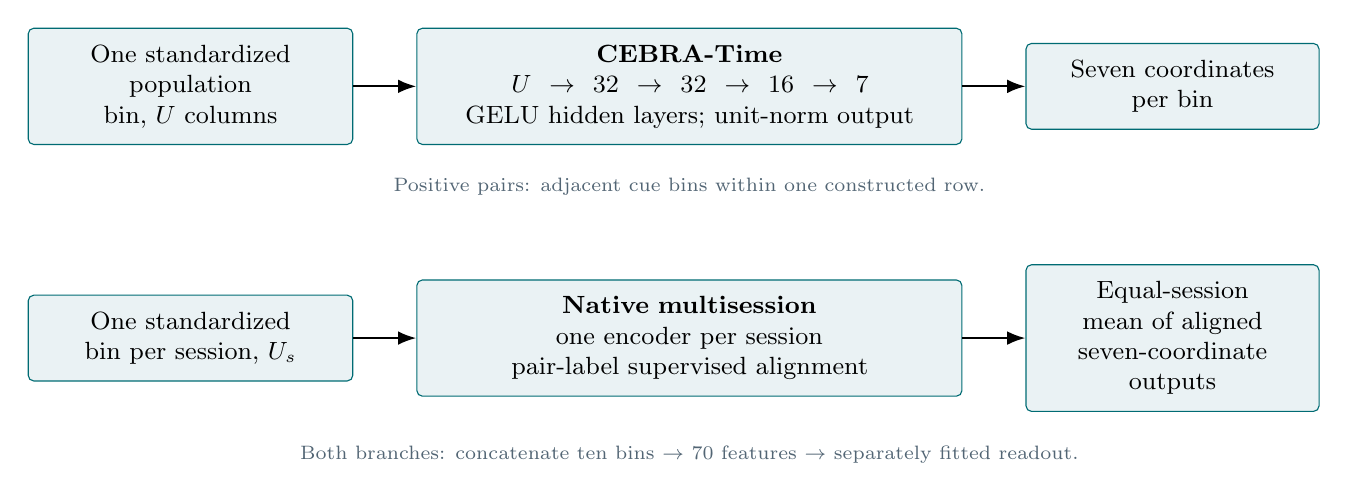
\begin{tikzpicture}[font=\small,>=Latex,
 b/.style={draw=accent,rounded corners=2pt,align=center,inner sep=6pt,fill=wash},
 arr/.style={->,thick}]
\node[b,text width=37mm] (x) {One standardized\par population bin, $U$ columns};
\node[b,text width=65mm,right=8mm of x] (time) {\textbf{CEBRA-Time}\par $U\to32\to32\to16\to7$\par GELU hidden layers; unit-norm output};
\node[b,text width=33mm,right=8mm of time] (z) {Seven coordinates\par per bin};
\draw[arr] (x)--(time);\draw[arr] (time)--(z);
\node[below=3mm of time,font=\scriptsize,text=muted] {Positive pairs: adjacent cue bins within one constructed row.};
\node[b,text width=37mm,below=19mm of x] (xs) {One standardized\par bin per session, $U_s$};
\node[b,text width=65mm,right=8mm of xs] (native) {\textbf{Native multisession}\par one encoder per session\par pair-label supervised alignment};
\node[b,text width=33mm,right=8mm of native] (pool) {Equal-session\par mean of aligned\par seven-coordinate outputs};
\draw[arr] (xs)--(native);\draw[arr] (native)--(pool);
\node[below=5mm of native,font=\scriptsize,text=muted] {Both branches: concatenate ten bins $\to$ 70 features $\to$ separately fitted readout.};
\end{tikzpicture}
\caption{Actual latest-study CEBRA pipelines (schematic). Time uses one network; native uses 3/11/20 session-specific networks as rosters expand. The latter also changes supervision, pooling and batch allocation, so it is not an isolated test of a software mode. Each branch uses 1,000 updates, learning rate $3\times10^{-4}$ and cosine temperature 1. Architecture and operations are visible in the executed notebooks \cite{latest,reproduction}.}
\label{fig:models}
\end{figure}

CEBRA optimizes a contrastive objective: specified positive pairs are favored relative to sampled negatives \cite{cebra}. Writing $z=f_\theta(x)$ and $s$ for cosine similarity, its learning principle can be expressed schematically as
\begin{equation}
 \mathcal L=-\mathbb E\,[s(z,z^+)/\tau]
 +\mathbb E\left[\log\!\sum_{j\in\mathcal N}\exp\{s(z,z_j^-)/\tau\}\right].
\end{equation}
Here the positive-pair rule defines what similarity the optimizer is encouraged to retain. The expression omits implementation-specific batch normalization constants; it is not a recomputation of logged losses. Time uses within-row adjacent-bin positives without endpoint-label supervision in its objective. Native uses joint-pair labels and the CEBRA multisession API. Neither falling loss nor a separated three-dimensional plot is, by itself, successful held-development decoding. Their losses are not directly comparable across objectives and batches.

Each representation is evaluated with logistic regression, radial-basis support-vector classification (RBF-SVM), uniform five-neighbor classification (kNN5) and singular-value-decomposition linear discriminant analysis (SVD-LDA), separately for pair, start and goal. Readouts have training-only scaling. Logistic $C=0.01(144/N)$ and SVM $C=144/N$ keep $NC$ fixed when U3 reduces the training row count $N$; that does not equalize combinations or optimizer exposure. SVM uses balanced class weights and \texttt{gamma=scale}, without probability calibration. LDA is a supervised classifier, not an unsupervised geometry reference.

The primary metric is mean class recall,
\begin{equation}
\BA=\frac1K\sum_{k=1}^K\frac{C_{kk}}{\sum_j C_{kj}},
\end{equation}
where confusion rows are true classes and columns predictions. Uniform references are $1/9$ for pairs and $1/6$ for endpoint heads. Five matched source-label worlds permute whole-pair labels within session and split \emph{before} assembly and fitting. They test alignment descriptively; five worlds and three computational seeds are not a calibrated significance test or biological confidence interval.

\clearpage
\section{Results I: distinct sources help some pipelines; repetition is not necessary}
Figure~\ref{fig:scores} shows every observed repeat and label-world score for the SVM pair readout. This is a fixed readable slice across all four representations; the full published tables include every readout and target, and Figure~\ref{fig:width} checks all readouts for the width claim. Uncertainty in these plots is computational variation on an exposed construction, not variation across new animals, sessions or held-out cohorts.

\begin{figure}[h!]
\centering
\figurefile[width=\linewidth]{recent_svm.pdf}
\caption{Latest-study whole-cue pair balanced accuracy. Top: fixed 17-column/3-session source-budget arms and the U3 once-only control. Bottom: nested width arms at three sources per pool. Individual colored traces/points show the three paired observed seeds; gray crosses show all five source-label worlds at model seed 0. The emphasized trace is the observed mean; the horizontal reference is $1/9$. Every score uses the same fixed nine classes and 72 label-conditioned, historically exposed development rows at its roster; shared blocks match across widths. Table~\ref{tab:design} distinguishes measured sources from rows. No biological confidence intervals are shown. Extracted from the published notebooks, complete case-score tables \cite{latest,reproduction}.}
\label{fig:scores}
\end{figure}

At fixed width, Raw/SVM pair means rise from 36.57\% (B2) to 37.96\% (B3) to 59.72\% (B5). Time/SVM rises from 16.67\% to 34.72\% to 46.30\%. The most clearly separated sampled contrasts are Raw B5$-$B3 ($+21.76\pp$) and Time B5$-$B2 ($+29.63\pp$): each of the three observed paired changes exceeds all five corresponding label-world changes. This is a descriptive comparison with the sampled controls, not a universal minimum-source threshold or a p-value.

PCA/SVM varies much less across these budgets: 32.41/33.33/34.26\%. Native/SVM gives 25.00/29.63/28.70\%. Thus the same additional source budget is not equally useful to all representations. The experiment changes source diversity and multiplicity together, so it cannot assign the gain to one of those mechanisms alone.

The once-only control is especially informative. U3 has 27 constructed training rows and the same 81 selected source IDs as B3. Raw/SVM averages 40.74\% and PCA/SVM 40.28\%, with every observed score above all five corresponding label-world scores. Reusing these sources in B3 changes their means by $-2.78\pp$ and $-6.94\pp$; Time and native instead change by $+10.19\pp$ and $+3.24\pp$. None of these four B3$-$U3 contrasts separates all observed changes from the diagnostic range. Repetition is unnecessary for the observed Raw/PCA association and is not uniformly beneficial; once-only \emph{training assembly} does not make development rows independent or eliminate repeated optimization exposure.

\clearpage
\section{Results II: broader rosters favor PCA means, not every repeat or pipeline}
PCA/SVM mean pair balanced accuracy is 33.33\%, 68.06\% and 72.22\% for 17, 49 and 83 columns. The 17$\to$49 change is $+34.72\pp$ and all three paired changes exceed the five matched diagnostic changes. The final mean gain is only $+4.17\pp$ and is positive in \emph{one of three} repeats; the other two worsen. Its control range overlaps. Reporting only the increasing means would obscure that qualification.

\begin{figure}[h!]
\centering
\figurefile[width=0.94\linewidth]{width_readouts.pdf}
\caption{All fixed readouts for the primary pair target: mean width changes in percentage points over three paired computational seeds. Positive values favor the larger roster. These are summaries of matched saved contrasts, not confidence intervals. Every comparison holds the nine classes and three selected sources per session--class pool fixed, with 144 training/72 development pseudorows; added rosters change columns, sessions and total measured sources together. PCA's mean rises in both steps for every readout, but this does not imply every repeat improves. Complete per-seed and five-world contrasts accompany the paper's aggregate data \cite{latest}.}
\label{fig:width}
\end{figure}

The all-readout view rules out a claim based solely on the displayed SVM. Both PCA and Time mean pair accuracy increase at both steps for logistic, SVM, kNN5 and SVD-LDA; the trend is not unique to PCA. Raw results are readout-dependent: logistic rises 42.13$\to$63.43$\to$66.20\%, while SVM peaks at 49 columns, 37.96$\to$52.31$\to$46.30\%. The Raw/SVM decline from 49 to 83 occurs in all three repeats. Time/SVM rises 34.72$\to$35.65$\to$48.61\%; its final $+12.96\pp$ contrast separates all observed changes from the five matched diagnostic changes.

Native/SVM gives 29.63$\to$38.89$\to$27.78\%, and the native mean declines from 49 to 83 for all four readouts. For SVM, one large repeat-level loss dominates the mean decline while the other two changes are small gains. That behavior cannot identify a harmful session. Native changes from 3 to 11 to 20 networks, with 255/253/240 total references per update and equal-session pooling. There is no matched concatenated pair-supervised comparator or untrained-encoder control. Fixed 1,000-update training does not demonstrate convergence. These results concern the configured pipelines, not the general merits of multisession learning.

Why might PCA benefit? Its seven-dimensional projection can aggregate structured variation before supervised readout, but the present contrasts do not identify the responsible biological variable or mechanism. Wider rosters add sources and session composition, and readout regularization interacts with feature geometry. PCA is a strong comparator under this design; selecting it as a universal winner from repeatedly inspected development would exceed the evidence.

These width effects and errors cannot yet be attributed to lost place-field coverage. Compact cue sources omit authenticated spatial rate maps and occupancy, with no validated join to these exact retained units and a common maze coordinate system. Coverage is \emph{unknown}, not zero. The saved retained-column and error tables make the missing evidence explicit, but issues 29/30's spatial interpretation and selectivity criterion remain untested. No spatial analysis is added here.

\clearpage
\section{Errors, temporal views and what the averages conceal}
\begin{figure}[h!]
\centering
\figurefile[width=0.90\linewidth]{errors.pdf}
\caption{Count and row-normalized confusions for Wfull PCA/SVM, seed 0, whole cue. Seed 0 was specified before matrix extraction; it happens to have the highest Wfull PCA/SVM score (88.89\%), so this is a high-score illustration, not typical performance (all repeats: Figure~\ref{fig:scores}). Rows are true pairs; columns are predictions. Each class has eight constructed exposed-development rows (72 total); one error changes recall by 12.5 points. Counts are predictions on constructed rows, not independent natural trials. Source: published confusion explorer \cite{latest,reproduction}.}
\label{fig:errors}
\end{figure}

Better aggregate performance can coexist with substantial regressions. In the post-hoc best/worst descriptions, Raw/SVM B5 versus B2 improves seven classes and worsens two: class $1\to4$ gains 75 recall points while $2\to5$ loses 12.5. Time/SVM Wfull versus B3 improves seven classes but worsens two, including a 50-point loss for $6\to2$. These are means over three repeats, each with eight development rows per class. The pooled 24 predictions per class repeat the same development construction and are not 24 independent biological trials.

Time has three meanings here: concatenated \emph{whole-cue} prediction, separately trained \emph{same-window} readouts (Figure~\ref{fig:time}), and \emph{temporal generalization} with a fitted decoder frozen across other windows. Historical raw-LDA goal transfer existed; matched CEBRA temporal/cross-phase transfer remains unexecuted. The latest latent class-mean cue lines average constructed rows in unaligned model coordinates: they are neither maze paths nor simultaneous dynamics \cite{endpoint,latest}.

\begin{figure}[h!]
\centering
\figurefile[width=\linewidth]{historical_time.png}
\caption{Historical October endpoint same-window decoding, reproduced unchanged \cite{endpoint}. Distinct cohort: 195 units/58 sessions, 12,288/3,265 train/development sources, 480/240 label-conditioned pseudorows. Each 100-ms cue bin has its own logistic or raw-LDA readout; horizontal position is cue-relative bin midpoint. Curves show three-seed means and min--max ranges; dotted lines are uniform references, not null distributions. These are computational ranges, not biological intervals or a frozen-decoder transfer matrix. \repo{docs/reports/cebra-endpoint-time-readout-20261006/figures/time_balanced_accuracy.png}{Full-size figure and legend}.}
\label{fig:time}
\end{figure}



\clearpage
\section{Defensibility: what has been established and what has not}
The strongest result across the recent series is that some endpoint association survives once-only training assembly under the declared source separation. Repetition is therefore not a necessary explanation for every favorable score. The strongest design lesson is that distinct-source support, realized multiplicity, class requirements, session membership and decoder choice must be explicit parts of the assay. They cannot be summarized by ``number of trials'' or ``number of neurons.''

Four limits prevent a stronger biological interpretation. First, evaluation uses known endpoint labels to assemble populations; it does not test unknown-label natural trials. Second, development is historically exposed and reused, so a favorable comparison is exploratory rather than a pristine confirmation. Third, disjoint contributors do not guarantee independent sources: serial dependence, within-session clustering and repeated development blocks remain. Three computational seeds are not three biological replicates. Fourth, unverified simultaneity, selected-unit sampling and missing subject/anatomical information prevent claims about a representative biological population. Source-safe computation improves validity within the assay; it does not manufacture the missing acquisition evidence \cite{contract,data}.

The November 11 saved-result error follow-up adds a complementary caution. Deleted classes were unevaluated in the reduced tasks; they must not be assigned zero recall. The removed classes were not uniformly the hardest. Source reuse often accompanied errors, but fuller-pool reuse is algebraically tied to lower coverage, so that correlation does not identify a causal repetition penalty. Session-roster contrasts likewise do not diagnose individually bad sessions \cite{errors}. The latest fixed-class design removes class deletion from its comparisons, but cannot turn source participation in an erroneous row into an individual-source causal attribution.

\begin{table}[h!]
\caption{Claim boundary for the completed series. A missing demonstration is not evidence that the biological phenomenon is absent.}
\label{tab:claims}\small
\begin{tabularx}{\linewidth}{Y Y}
\toprule
Supported by the recorded analyses & Not established by these analyses \\
\midrule
Condition-level endpoint association in specified source-separated constructions. & Prediction on unknown-label natural trials; independent prospective biological generalization. \\
Pipeline-specific effects of selected source budget, reuse policy and roster expansion. & Pure causal effects of duplication, neuron count, or a particular cell/session. \\
Some favorable simple-feature comparisons and configured CEBRA results. & General PCA/CEBRA superiority; neural mechanism from a decoder or embedding. \\
Same-window decoding and descriptive latent class-mean trajectories where reported. & Matched frozen CEBRA temporal/cross-phase transfer; simultaneous dynamics or biological rotation. \\
Repeatable execution and authenticated saved results. & Independent biological replication; ordered-path recovery beyond endpoints; formal neural-state observability. \\
\bottomrule
\end{tabularx}
\end{table}

For the sparse nine-class task, even hypothetical perfect knowledge of only one endpoint permits pair balanced accuracy $6/9=66.67\%$: each of six endpoint categories can identify or distribute predictions over its associated pair classes, contributing a total recall of six. This is a mathematical reference, not a fitted neural baseline. Exceeding the uniform $1/9$ reference therefore does not isolate conjunctive coding or path information beyond endpoints. Even exceeding $6/9$ would not by itself establish biological conjunction, mechanism or route coding.

The recent reproduction strengthens the computational record. The six arms, three observed seeds and five diagnostic worlds make 48 unique cases: 2,448 model-fit calls excluding scalers and 96,000 CEBRA updates per complete execution. The fuller notebooks expose first-case training and complete 38 code cells. Independent checks authenticate 3,188 run files; 14,304 saved numerical arrays exactly match the accepted execution, and all 96 learning records agree apart from wall time. The earlier kernel-handoff failure, reviewed continuation and failed software checks remain preserved \cite{reproduction}. Matching this computation on the same recordings and seeds is reproduction, not another sample from biology.

The series has progressed toward a more inspectable conditional assay. A reusable hippocampal task-state representation remains an ambition, not a delivered model. Formal observability asks whether a specified dynamical model's state can be recovered from its measurements; readable computation and successful label prediction do not establish it. The present contribution is an explicit link from measurements and construction to prediction and claim, retaining positive and negative results. This synthesis initiates no new study.

\clearpage
\section*{Evidence, reproducibility and references}
The accompanying source package contains this LaTeX manuscript, vector figures, full-precision extracted aggregate score/contrast tables, a figure-building script and a source-hash manifest. Figures are presentation-level recomputations from public notebook tables, with shared B3 records deduplicated by identity; no fitted objects or trial-level neural arrays are required. The source revision is pinned in the repository links below. Detailed methods, complete controls and original provenance remain in their owning study records rather than being silently harmonized across cohorts.

The three requested manuscript audits are recorded separately with the exact reviewed PDF/source hashes. They are independent AI-agent reading and evidence audits (newcomer, experienced researcher and quantitative/provenance reviewer), not journal peer review or external biological replication. The paper's source tables permit independent checking of the latest displayed numbers without accepting its narrative on authority.

\begingroup\small
\begin{thebibliography}{99}
\setlength{\itemsep}{4pt}
\bibitem{history} Neuroscience workspace. \repo{history/README.md}{Weekly research history and study records}, July--October 2026; \repo{docs/reports/cebra-research-synthesis-20261011.md}{research synthesis plan}. Historical results retain their original targets, splits and controls.
\bibitem{path} Neuroscience workspace. \repo{docs/reports/path-generalization-completed-state-20260907.md}{Completed path-generalization study}; \repo{docs/professor_updates/path_generalization_20260907/CORRECTIONS.md}{correction ledger}. Source-recombination and exact development-product evaluations are distinct.
\bibitem{contract} Neuroscience workspace. \repo{docs/analysis-contract.md}{Analysis contract}; \repo{docs/project-direction.md}{agreed project direction}. Source identity, contributor separation, target distinctions and condition-level claim boundaries.
\bibitem{data} Neuroscience workspace. \repo{docs/dataset-card.md}{Dataset and experimental-setup reference}; \repo{data/README.md}{compact cue-source contract}; \repo{context/previous-student-analysis.md}{prior-student analysis summary}. Dated evidence labels distinguish observed, code-established and unresolved acquisition details.
\bibitem{endpoint} Neuroscience workspace. \repo{docs/reports/cebra-endpoint-time-readout-20261006/README.md}{Endpoint and cue-time readout report}, accepted October 7, 2026; \repo{report/README.md}{saved-artifact review notebook and replay boundaries}, October 19.
\bibitem{fresh} Neuroscience workspace. \repo{docs/reports/cebra-27unit-notebooks-20261023/README.md}{27-unit cue-only notebook study}, executed October 23, 2026; report published November 2. Two computational seeds and one permutation diagnostic.
\bibitem{support} Neuroscience workspace. \repo{docs/reports/source-support-ablation-20261110/README.md}{Endpoint learning after reducing classes and source reuse}, November 10, 2026; \repo{docs/source-support-protocol-20261110.md}{frozen protocol}.
\bibitem{grid} Neuroscience workspace. \repo{docs/reports/population-grid-20261111/README.md}{Class requirements, session rosters and learning}, November 11, 2026; \repo{docs/population-grid-protocol-20261111.md}{protocol}. 111 cases, 5,661 model fits and 222,000 updates; distinct from the latest 48-case design.
\bibitem{errors} Neuroscience workspace. \repo{docs/reports/population-grid-20261111/error-analysis.md}{Saved-result confusion, class-deletion and source-reuse analysis}; \repo{docs/reports/population-grid-20261111/error-analysis-validation.md}{validation}. Prediction-only follow-up; no new fitting.
\bibitem{latest} Neuroscience workspace. \repo{docs/experiments/source-reuse-width-20261114/README.md}{Source reuse, then population width: results}; \repo{docs/experiments/source-reuse-width-20261114/protocol.md}{frozen protocol}; \href{https://github.com/Hong-yiii/neuro_science/pull/31}{PR 31}. Defined November 14; executed and delivered November 15, 2026.
\bibitem{reproduction} Neuroscience workspace. \repo{docs/experiments/source-reuse-width-20261114/notebook-validation-20261115.md}{Complete notebook reproduction and validation}; \repo{experiments/source_reuse_width_20261114/walkthrough_20261115/published/manifest.json}{published artifact manifest}. Two complete executed notebooks; explicit post-execution editorial correction and saved-figure supplement.
\bibitem{cebra} Schneider, S., Lee, J. H. and Mathis, M. W. Learnable latent embeddings for joint behavioural and neural analysis. \emph{Nature} \textbf{617}, 360--368 (2023). \href{https://doi.org/10.1038/s41586-023-06031-6}{doi:10.1038/s41586-023-06031-6}. Method reference inherited from the existing manuscript, not evidence for this dataset's biological claims.
\bibitem{dimred} Cunningham, J. P. and Yu, B. M. Dimensionality reduction for large-scale neural recordings. \emph{Nature Neuroscience} \textbf{17}, 1500--1509 (2014). \href{https://doi.org/10.1038/nn.3776}{doi:10.1038/nn.3776}. Existing methodological context for interpreting derived coordinates.
\end{thebibliography}
\endgroup
\end{document}
